% The entire content of this work (including the source code
% for TeX files and the generated PDF documents) by 
% Hongxiang Chen (nicknamed we.taper, or just Taper) is
% licensed under a 
% Creative Commons Attribution-NonCommercial-ShareAlike 4.0 
% International License (Link to the complete license text:
% http://creativecommons.org/licenses/by-nc-sa/4.0/).
\documentclass{article}

\usepackage{float}  % For H in figures
\usepackage{amsmath} % For math
\usepackage{amssymb}
\usepackage{bbm} % for numbers within mathbb
\usepackage{mathrsfs} % For \mathscr{ABC}
% Followings are for the special character: differential "d".
\newcommand*\diff{\mathop{}\!\mathrm{d}}
\newcommand*\Diff[1]{\mathop{}\!\mathrm{d^#1}}
\numberwithin{equation}{subsection} % have the enumeration go to the subsection level.
                                    % See:https://en.wikibooks.org/wiki/LaTeX/Advanced_Mathematics
\usepackage{graphicx}   % need for figures
\usepackage{cite} % need for bibligraphy.
\usepackage[unicode]{hyperref}  % make every cite a link
\usepackage{CJKutf8} % For Chinese characters
\usepackage{fancyref} % For easy adding figure,equation etc in reference. Use \fref or \Fref instead of \ref
\usepackage{braket} %http://tex.stackexchange.com/questions/214728/braket-notation-in-latex

% Following is for theorems etc environments
% http://tex.stackexchange.com/questions/45817/theorem-definition-lemma-problem-numbering && https://en.wikibooks.org/wiki/LaTeX/Theorems
\usepackage{amsthm}
\newtheorem{defi}{Definition}[section]
\newtheorem{thm}{Theorem}[section]
\newtheorem{lemma}{Lemma}[section]
\newtheorem{remark}{Remark}[section]
\newtheorem{prop}{Proposition}[section]
\newtheorem{coro}{Corollary}[section]
\theoremstyle{definition}
\newtheorem{ex}{Example}[section]

% A list of nomenclatures.
\usepackage{nomencl}
\makenomenclature

\usepackage[all]{xy} % For drawing diagrams with arrows
\title{Notes of Connecting Few-body and Many-body Pictures of Fractional Quantum Hall Physics}
\date{\today}
\author{Taper}


\begin{document}


\maketitle
\abstract{
    I wrote this with the aim of finding some interesting topics for
    research. This conference has its lecture recorded and published
    in YouTube (link\cite{utube-lecture}).
    Note that, although I have the video on hand, the lecturers are
    speaking somehow too fast and it would be too time-consuming to replay
    these lectures. So the content is..... quite un-organised and bare.
    In addition, after typing for several hours, my fingers are getting
    tired. So... I could be very lazy.

    Therefore, this note could be viewed just as a collection of keywords.
}
\tableofcontents
\section{Using Optical Emission to Study Competing Phase in the Second
Landau Level}
\label{sec:Using-Optical-Emission-to-Study-Competing-Phase-in-the-Second-Landau-Level}

By: 

Antonio Levy, Aron Pinczuk, Yuliya Kuznetsova (Columbia University),
Ursula Wurstbauer (Technische Uni. Munchen), Ken. W. West, Loren N.
Pfeiffer (Princeton), Michael J. Manfra, Geoff C. Gardner, John D. Watson
(Purdue University).

\paragraph{Overview} Second Landau Level displays
\begin{enumerate}
    \item FQHS
    \item Ordered phases (partially). RIQHE $ \overset{from}{\Leftarrow}$
        Electron stalids.
    \item Competition \& Coexistance

        Anisotropic FQHS arise from coorelation when anisotropic
        $\overset{from}{\Leftarrow}$ magneti field
\end{enumerate}
\paragraph{Advanage of Optial}
\begin{enumerate}
    \item Direct probes bulk
    \item Distinguish between charge and spin modes
\end{enumerate}
\paragraph{Sample} Omitted.
\paragraph{RRS}
$ $ % Go to the next line.

$ \xymatrix{
    \text{light}\ar[r] &
    \bullet\ar@/^/[r]^{\text{quasiparticle}}
                \ar@/_/@{<.}[r]_{\text{quasihole}} & 
    \bullet & \text{scattered photon}
}$

$\bullet$ Easy to probe Single Partical excitation and collective
excitation.

... (Skipped)

\section{Hyperspherical Adiabatic Approximation}
\label{sec:Hyperspherical-adiabatic-Approximation}

By: Rachel Wooten (Purdue University)

\paragraph{Outline}
\begin{enumerate}
    \item QHS
    \item Motivation
    \item Hyperspherical adiabatic approximation (\textbf{HAA})
    \item The role of degeneracy
    \item Hyperradial breathing mode
    \item Results and Discussion
\end{enumerate}

\paragraph{QHS}
\begin{table}[H]
    \caption{Two Schemes}
    \centering
    \begin{tabular}{|ccc|}
        \hline
        Conventional     & $\approx$ & Neutral Atom gass \\
        \hline
        2D Landau levels &           & 2D Rotation($\Omega$) \\
        $\omega_c$       &           & $\omega= 2\Omega$ \\
        \hline
    \end{tabular}
\end{table}

(Other schemes are also available, not treated).

\paragraph{Motivation}
\begin{itemize}
    \item QHS: prototype of \textit{Strongly correlated systems}
    \item Nature of few-body states
    \item insights from collectively coordinates
    \item use ... ?
\end{itemize}

\paragraph{Few body, adiabatic hypershperical approach\textbf{(AHA)}}

\begin{itemize}
    \item intrinsic collective coordinates
    \item length scale $R$ $\overset{\text{from}}{ \Leftarrow}$ geometry
    \item $E$ potential $ \Leftarrow$ length scale
    \item introduce Grand Angular momentum $K$ - quantum number
\end{itemize}

\paragraph{AHA background} Joe Macek, 1968 JPB.

\paragraph{Scheme} Sch-Ep $\overset{recast}{ \Rightarrow}$ relative
coordinates $ \overset{diagonalize}{ \Rightarrow}$ solve.

\paragraph{Hyperspherical Coordinates} $ $

$2N-2$ Jacobi coordinates $\Rightarrow$ $2N-3$ angular coordinates
$\Omega$ + 1 length coordinates Hyperradial $R$.
\begin{figure}[H]
    \centering
    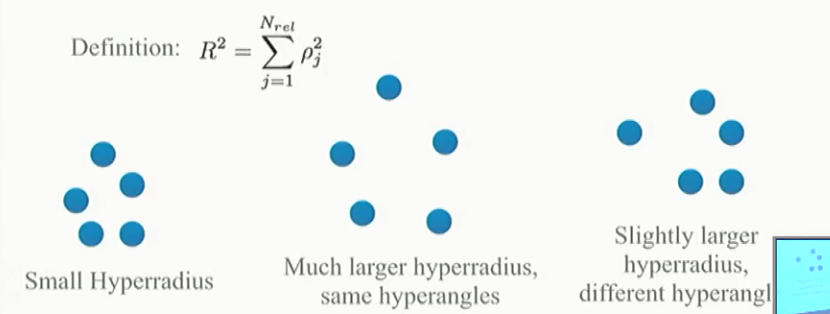
\includegraphics[width=0.8\linewidth]{pics/rachel-wooten-purdue.png}
\end{figure}

\paragraph{Hyperradius}
$$\rho = \left( \frac{\pi\mu\braket{R^2}}{N(N-1)} \right)$$
$$\mathscr{H}_\text{rel} = (R, \Omega, \cdots)
    +\text{Colomb} V(R)=\frac{1}{R}
    +\text{Polarized dipoles}V(R)=\frac{1}{R^3}
$$
\paragraph{AHA (Non-interacting case)} Omitted.
\paragraph{AHA (Interacting case)}$ $

Treat $R$ as an adiabatic parameter. 

Interaction $\overset{\text{introduct}}{\Rightarrow}$ degeneracies
\paragraph{Accuracy check} Omitted.
\paragraph{Exceptional degeneracy}

\section{? (Wick Haxton)}
\label{sec:Wick-Haxton}

(1995) Algebraic classification of general 4 fermion problem (Joe
Ginocchio) $\Rightarrow$ has FQHE implications

Jain \& Laughlin work (numerically succesful)

(No audio available for this lecture recording!, Skipped)

\section{Perspectives on the half-fill Landau Level}
\label{sec:Perspectives-on-the-half-fill-Landau-Level}

By B.I. Halperin, N. Copper, Chong Wong, Adey Stern.

\paragraph{Question}: What ahppens to half-filled Landau Level when there
is \textbf{NO} magnetic field.

\paragraph{Motivation}
\begin{itemize}
    \item New research on half-filled Landau level
    \item Describe system by "Dirac Fermion" is simpler, generated
        different theories $\Rightarrow$ doubt whether they are
        equivalent.
    \item Particle-hole symmetry in explicit in "Dirac Fermion", not
        explicit in HLR framwork.
\end{itemize}
\paragraph{Physical Setup} $ $

Half-filled Landau level: in a semiconductor.
$$ H_0 = \sum_i \frac{ |P_i - A(r_i)|^2}{2m} + V_2 \text{(interactions)}
$$
Units: $e=\hbar=1$.
\paragraph{PH Symmetry} $ $

\begin{itemize}
    \item $m\to 0$, e-e interactions are fixed -> exact PH symmetry
    \item For $v=1/2$, PHS requires that $\sigma_{xy}(\sigma)=(1/2) e^2/h$
\end{itemize}

\paragraph{HLR Approach}
(Halperin, Lee, Read. PRB 1993)

\begin{itemize}
    \item Singular gauge transformation $\Rightarrow$ Chern-Simons Gauge
        Field
    \item Transformed Hamiltonian will have fermion terms, interactions,
        gauge field (chern-simons interaction in it). Also the curl of a
        fact vector is constrained.
\end{itemize}
\paragraph{Antecednets}
\begin{itemize}
    \item Fractional Quantized Hall states by Jain; Lopez and Fradkin;
        others.
    \item Simultaneous work by Kalmeyer and Zhang had some features of
        HLR.
\end{itemize}

\paragraph{HLR Hypothesis}
\begin{itemize}
    \item Do mean field theory on this problem: the ground state and low
        energy properties of quantum hall system at $v=1/2$. And use
        perturbation theory and take into account of fluctuations in gauge
        field and Coulomb interactions
    \item ...
\end{itemize}
\paragraph{HLR consequences}
\begin{itemize}
    \item with $1/r$ interactions, the ground state is a "marginal fermi
        liquid". With mass diverges $log$ at fermi serface, eue to
        infrared divergence.
    \item assume interactions that fall off slower than $1/r$.
\end{itemize}
\paragraph{HLR-RPA predications}
\begin{itemize}
    \item ground state at $v=1/2$ should be compressible
    \item energy gaps, FQH states, occur at Jain fractions $v=p/(2p+2)$.
    \item relative sizes of energy gaps close to $1/2$
    \item transport in absence of impurities: DC hall conductance
    \item Longitudianl conductivity at finite $q,\omega\to 0$:
        $$\sigma_{xx}(q)=q/(8\pi k_f) $$
        in the presence impurities: formula holds for $q>l_{cf}$.
\end{itemize}
\paragraph{HLR-RPA problems}
\begin{itemize}
    \item most important error: ignores renormalization of fermian
        effective mass. gives wrong energy scale, wrong value for specific
        heat at $1/2$, wrong scale for FQHE gaps.
    \item correct effective mass is set by the e-e interaction, not by the
        bare mass, when $m$ is small.
\end{itemize}
\paragraph{Naive renormalizaed RPA}
\begin{itemize}
    \item simply replace $m$ by $m^*$.
    \item however: iolates Kohn's theorem for $\omega=\neq 0$.
    \item and many many....
\end{itemize}
\paragraph{Landau interaction parameters}
\begin{itemize}
    \item energy cost of a ditortion of fermi surface, independent of
        position.
    \item (several formulae)
\end{itemize}
\paragraph{DC conductitivity in presence of impurties}
\begin{itemize}
    \item Kivelson (1997): naive HLR leads to deviations
    \item ... continued of problems of HLR-RPA
\end{itemize}
\paragraph{Side-jump contribution} ......
\paragraph{Commensurability oscillations: $v\neq 1/2$, with finite $q$}
and this result is symmetric w.r.t $\Delta B$, different from HLR.

\section{Composite fermi liquids in the lowest Landau level}
\label{sec:Composite-fermi-liquids-in-the-lowest-Landau-level}
By: T. Senthil (MIT), Chong Wang (MIT -> Harvord)

\paragraph{2d electrons in the QH regime}
\footnote{This is the first time that I find a correct usage of the word
"regime", without suspicion that it should be replaced by "region".}.
\paragraph{Unquantized region}

\begin{itemize}
    \item Incompressible FQHE states: fill certain rational fractions of a
        Landau level
    \item Large degeneracy is split by e-e interactions to give a gapped
        ground state
    \item compressible metallic states: "unquantized
        quantum Hall effect"
    \item \textbf{How do interactions manage to produce a metal}
\end{itemize}

\paragraph{Standard theory} HLR theory, idea of composite fermions

\paragraph{Some experimental verification of composite fermions}

\paragraph{Unsatisfactory aspects of the theory}
\begin{itemize}
    \item HLR not suited to projecting to Lowest Landau Level (LLL)
    \item mean field effective mass = bare electron mass
    \item LLL limit: take $m$ to zero: what happens?
    \item LLL theory has an extra symmetry that HLR is blind to. the PH
        symmetry.
\end{itemize}
\paragraph{PH symmetry: formal implementation} ways to exam the
particle-hole symmetry.

Numerical work: shows metallic ground state $v=1/2$ preserves the C
symmetry.

HLR theory: not in LLL, therefore it does not address the problem of p/h
within its scope.

\paragraph{Related theoretical problems}
\begin{itemize}
    \item electrons at $v=1/4,1/6,\cdots$ No p/h. But issue of nature of a
        LLL theory remains
    \item useful to consider problem of bosons in the quantum Hall regime.
        Fate of such a state in LLL. For bosons, microscopically there is
        no p/h.
\end{itemize}
\paragraph{Progress old and new}
\begin{itemize}
    \item Bosons at $v=1$: LLL theory of metallic Composite Fermi Liquid
        (\textbf{CFL}) state (Read 1998)
    \item PH symmetric theory for electronc CFL at $v=1/2$.
        by Son (2016): Is the composite fermion at $v=1/2$ a dirac
        particle?
        \begin{itemize}
            \item field theoretic justification: connection to the surface
                of 3d topological insulators (C. Wang. TS ...)
            \item Simple physical picture of the PH symmetric composite
                fermion (C. Wang. ...)
            \item Numerical calculations (...)
        \end{itemize}
\end{itemize}
\paragraph{Talk outline}
\begin{itemize}
    \item Understanding the p/h symmetric composite fermi liquid of
        electrons at $v=1/2$ (physical picture, field theoretic
        derivation)
    \item Composite Fermi Liquid of bosons at $v=1$:
        \begin{itemize}
            \item review of Read's Lowest Landau Level theory
            \item comparison with electrons at $v=1/2$.
        \end{itemize}
    \item Composite Fermi Liquids in LLL at generic $v$:
\end{itemize}
\paragraph{Old physical picture Composite Fermion in LLL}
LLL wave function: (Rezayi-Read 94)
$$ \psi= P_{LLL} \mathrm{det}(e^{ik_i r_j})\prod_{i<j} (z_i-z_j)^2 $$
Composite fermion = electron bound to $4\pi$-vortex which has charge
depletion $-e$. They are neutral but carry a dipole moment.

Howeer this picture misses some physics and further is not PH symmetric.

\paragraph{New picture of composite fermion in LLL}
by Wang. TS.
$$\psi=\prod_{i<j} (z_i-z_j)f(z_1,\cdots,z_N)$$
where $f$ is symmetric.

One vortex is exactly on electron due to Pauli. Each vortex has charge
$-e/2$ => single vortex exactly on electron has charge $+e/2$ and the
displaced vortex has chare $-e/2$.

\paragraph{Internal structure of composite fermion in LLL}
Two ends have mutual statistics of $\pi$. Solve Quantum Mechanics of just
relative motion. $\cdots$

\paragraph{1/2-filled LL and correlated 3 dimentional Topological
Insulator surface} Derivation of and more
insidght into PH symmetric composite fermi liquid theory.

Skipped.

\section{Nematic order in fractional quantum Hall liquids}
\label{sec:Nematic-order-in-fractional-quantum-Hall-liquids}
By Joseph Maciejko (University of Alberta).

\paragraph{FQH nematic}
\begin{itemize}
    \item A proposed novel state of matter where (topological) FQH order
        coexists with (conventional) nematic order
    \item Intrinsic topological order (blobal) is insensitive to symmetry
        considerations (local); Can imaagine many possible broken
        symmetries.
    \item ...
\end{itemize}
\paragraph{FQH nematic at $v=7/3$} Xia et al., Nat. Phys. 2011.

\paragraph{FQH nematic at $v=5/2$} Samkharadze et al., Nat. Phys. 2015.

No symmetry breaking field, but not clear if there is a Hall plateau or
not

\paragraph{FQH nematic at $v=5/2$} Liu et al., PRB 2013 No Hall plateu
reported, but longitudinal resistances appear to vanish as $T\to 0$.

\paragraph{Disclaimer}
\begin{itemize}
    \item Some of these experiements may or may not be explained by a FQH
        nematic
    \item will focus on FQH nematic
    \item theoretical: Haldane's geometrical perspective on the FQHE.
\end{itemize}
\paragraph{FQH isotropic-nematic transition}
\begin{itemize}
    \item Main questions
        \begin{itemize} 
            \item Generic mechanism for a transition from
            isoropic FQHE to FQH nematic 
            \item effective field theory of
            the transition?  
            \item can we realize this transition in a
            microscopic model of interacting electrons?  
        \end{itemize}
    \item isotropic FQH liquid is naturally proximate to a FQH nematic
    \item Girvin-MacDonald-Platzman (GMP) mode in the $q=0$ limit
        corresponds to gapped nematic fluctuations wich condense at a
        putaative isotropic-nematic QCP (JM et al., PRB 2013).
\end{itemize}

\paragraph{GMP mode} "Intra-LL" neutral collective mode in the FQHE (by
contrast with "inter-LL" Kohn/magnetoplasmon mode). G. M. P., Prl 1985.

$q=0$ limit of GMP mode has quadrupolar symmetry
\paragraph{GMP mode as a quadrupole}

\begin{itemize}
    \item numerical studies $\cdots \cdots$.
    \item heuristic argument.
\end{itemize}
\paragraph{geometrical theory of the FQHE}
\begin{itemize}
    \item $q=0$ limit of the GMP = fluctuating intrinsic "metric"
        $g_{ab}(r,t)$ (Haldane PRL 2011; ....)
    \item Metric is unimodular ($\mathrm{det} g = 1$): set of ellipses of
        fixed area, i.e., quedrupolar deformations of the circle.
\end{itemize}
....
\paragraph{Intrinsic metric and nematicity}
\begin{itemize}
    \item Unimodular metric equivalent to nematic order parameter
        $Q_{ab}$.
\end{itemize}
$$ g = \mathrm{exp}Q$$
$\cdots$

\paragraph{FQH isotropic-nematic transition} $\cdots$
Skipped.

\section{Rotational properties of multi-species Bose gases}
\label{sec:Rotational-properties-of-multi-species-Bose-gases}

By Suasanne Viefers, University of Osio.
\marginpar{A good one for those not familiar with this field.}
\paragraph{Outline}
\begin{itemize}
    \item Review of rotating bosons in the LLL quantum Hall connection
    \item Two- and three- species Bose gases
    \item Composite fermion approach: results and puzzles
    \item outlook
\end{itemize}

\paragraph{Rotating Bose condensates}
\begin{itemize}
    \item 1995: first atomic Bose condensate
    \item 1999: first vortex in rotating BEC (JILA, Paris)
    \item 2004: Abrikosov lattice in Lowest Landau Level (200 vortices)

        Increasing rotation: cloud flattens out, density decreases, weaker
        interaction, lowest Landau level.

        Eventually: Vortex lattice predicted to melt, so system enters
        quantum Hall regime
    \item Recent reports of small systems ($N<10$) reaching FQH regime in
        novel type of optical lattice with local rotation of each site.
\end{itemize}

\paragraph{LLL wave functions}
\begin{itemize}
    \item Historical motivation: Quantum Hall effect
    \item 2-dimensional electron gas in a strong perpendicular magnetic
        field at low T
    \item Electrons residing mainly in the LLL
\end{itemize}

Construction of explicit trial wave function by various schemes (in
partular) Laughlin, hierarchy/composite fermions) has proven very
successful in exploring QH physics. Not exact, but o capture essential
properties (topological order).

\paragraph{Bose condensate in the LLL}
Mathematical equivalence in 2D between rotation (harmonic oscillator) and
perpendicular magnetic field.

In the absence of interaction: Lowest N-body state with give $L$ is highly
degenerate. The interaction lifts this degeneracy and selects the lowest
("yrast") state. (Yrast= "most dizzy"). \footnote{Here is one anecdote.}

\begin{itemize}
    \item N-particle state: symmetric homogeneous polynomials.
    \item Total angular momentum = deree of polynomial
\end{itemize}

Composite fermion scheme modified and shown to work successfully for the
entire yrast line, including low angular momenta.

\paragraph{Multi-component systems} ...
\paragraph{Two component systems: QH regime}
\begin{itemize}
    \item Two species Bose gases in the quantum Hall regime: several
        theoretical studies.
    \item Proposed (under discussion): NASS state at $v=4/3$.
    \item Fundamentl quasiholes: charge $e/3$ non-Abelian anyons
    \item Bosonic IQH states with topologically protected edge states.
\end{itemize}

\paragraph{Two-component systems: Slow rotation}
\begin{itemize}
    \item Study 2-species Bose gas in LLL with homogeneous contact
        interaction.
    \item Recent work identified a class analytically exact many-body
        eigenstates for low angular momenta
    \item Beyond papenbrock? Study low $L$ regime in terms of composite
        fermions, exploiting (pesudo) spin analogy for homogeneous
        interaction. Not a priori expected to work
    \item Choice of Slater determinants in general not unique, i.e.
        several $CF$ candidates -- may or may not be lineary dependent.
\end{itemize}
\paragraph{Simple example}...

\paragraph{Selection criteria for Slaters}...
\paragraph{Full CF diagonalization}
\paragraph{Sample states}...
\paragraph{Puzzles: linear dependencies}

\begin{itemize}
    \item the number of apparent CF condidates is generally too large,
        after projection.
    \item This is true even when restricting to simple states.
    \item Similar problems were recently discussed in the context of
        higher bands for electronic FQH states. without fully succeeding
        to reveal the underlying mathematical structures
    \item ...
    \item Wish: identify linear dependdencies before projection (for
        numerical concern).
\end{itemize}
\paragraph{Linear dependencies (simple states): Ingredients} ...
\begin{itemize}
    \item More direct understanding of linear dependencies in the CF
        formalism?
    \item Go beyond homogeneous interaction, study vortex structures,
        anyonic quasiparticles in QH regime
    \item Future experiments in this regime?
    \item Spin-I
    \item NORDITA program "topological phases in cold atom systems" Aug
        2017.
\end{itemize}

\section{Artificial gauge fields with ultracold bosonic atoms in optical
lattices}
\label{sec:Artificial-gauge-fields-with-ultracold-bosonic-atoms-in-optical
lattices}
By Monika Aidelsburger (LMU Munich, MP institute of Quantum Optics).

\paragraph{Outline}
\begin{itemize}
    \item Realization of artificial magnetic fields using laser-assisted
        tunneling
    \item Experimental results
    \item Chern-number measurement
    \item Summary and prospects
\end{itemize}
Skipped. May contain a good introduction to topological Insulator
concepts. But I have really limited amount of time now.

\section{Generalized Topological Forces}
\label{sec:Generalized-Topological-Forces}
By I.B. Spielman (JQI - Maryland).

\paragraph{Topology in CMP}
How the underlying topology gives rise to the forces.
\paragraph{Outline}
\begin{itemize}
    \item Geometric charge pumping

        From abelian Berry's curvature related to the 1st chern
        number/class.
    \item 2nd Chern number/class

        From non-abelian Berry's curvature.
\end{itemize}
\paragraph{Pumps throughout history} From archimedean to NIST single
electron pump. 

\paragraph{Questions from simple 1D lattice}
A force "just" causes Bloch oscillations.
\begin{itemize}
    \item Gives motion in topological/geometric pumps 
    \item Deflects trajectories in Bloch oscillations
    \item Force underlying quantum Hall effect
\end{itemize}

\paragraph{Topology in parameter space}
\paragraph{Monopole - topological defects}

He seems to want to create some concepts of force in CMP system. And I
decided to skip him for the moment.
\section{Anchor}
\label{sec:Anchor}

\begin{thebibliography}{1}
    \bibitem{utube-lecture}\url{https://www.youtube.com/playlist?list=PLCoSh1h28ieLIaD-HGi5aUQzunOTtxHTC}
\end{thebibliography}
\printnomenclature
\section{License}
The entire content of this work (including the source code
for TeX files and the generated PDF documents) by 
Hongxiang Chen (nicknamed we.taper, or just Taper) is
licensed under a 
\href{http://creativecommons.org/licenses/by-nc-sa/4.0/}{Creative 
Commons Attribution-NonCommercial-ShareAlike 4.0 International 
License}. Permissions beyond the scope of this 
license may be available at \url{mailto:we.taper[at]gmail[dot]com}.
\end{document}
